\section{Güte, Validierung und Verallgemeinerbarkeit}
\label{sec:validierung}

In den vorangegangenen Unterkapiteln habe ich meine \gls{gt} vorgestellt. Für die darin beschriebenen Usability-Probleme habe ich Lösungsmaßnahmen vorgeschlagen und deren Bearbeitung durch die SeqAn-Entwickler beschrieben.

In diesem Unterkapitel möchte ich die Fragen beantworten, inwiefern meine Forschung überhaupt den Gütekriterien qualitativer Forschung entspricht und ob die Umsetzung meiner vorgeschlagenen Maßnahmen tatsächlich zu der erhofften Usability-Verbesserung führten. Des Weiteren möchte ich die Frage nach der Verallgemeinerbarkeit meiner Forschungsmethode und -ergebnisse klären.

\subsection{Güte}

In dieser Arbeit habe ich einen qualitativen Forschungsansatz gewählt, bei dem die \gls{gtm} eine große Rolle spielt. Für die Bewertung der Güte meiner Arbeit gelten also die am Anfang dieser Arbeit, im \sref{sec:gtm}, vorgestellten Gütekriterien qualitativer Forschung. Entlang dieser Gütekriterien werde ich meine Arbeit bewerten.

\begin{description}
  \item[Verfahrensdokumentation] \hfill \\
  Ich habe meine durch die wissenschaftliche Literaturstudie erworbenen Vorkenntnisse, die Forschungsplanung, die Datenerhebung, den Bau des Datenanalysewerkzeugs, die Herleitung der \gls{gt}, das Zustandekommen der Verbesserungsvorschläge und deren Umsetzung ausführlich beschrieben. Dabei habe ich die erhobenen Daten und die Grundlagen der von mir entwickelten Konzepte detailliert mittels entsprechender URIs zugänglich gemacht. Durch den Einsatz einer Versionsverwaltung kann sogar das Zustandekommen meiner als XML-Datei gesicherten Theorie über die Zeit nachvollzogen werden.
  
  \item[Argumentative Interpretationsabsicherung] \hfill \\
  Aus Platz-, Zeit- und Plausibilitätsgründen habe ich der Darstellung von Interpretationsalternativen nur wenig Raum in dieser Arbeit gegeben. Wenn es zu Konzepten relevante Literatur gab, habe ich diese genannt und zu meinen Beobachtungen in Beziehung gesetzt. Hatte ich Unsicherheiten in der Interpretation von Konzepten, habe ich diese bei für wichtig geglaubten Konzepten ausgeräumt. Weniger wichtige Konzepte habe ich in dieser Arbeit nicht aufgeführt. Die schlecht verstandenen Konzepte (z.B. \code[apiua://code/-9223372036854775057]{versteckte Parameterübergabe}) habe ich als solche deklariert.
  
  \item[Regelgeleitetheit] \hfill \\
  Meine Forschungsergebnisse entstanden innerhalb eines Prozesses, der stark durch die \gls{gtm} geprägt war. Durch die Implementierung eines dazugehörigen Analysewerkzeugs habe ich insbesondere die Phasen des offenen und axialen Kodierens und damit einen umfangreichen Prozessteil kodifiziert. Bei meiner Forschung kam es zu Abweichungen, die ich nachvollziehbar erläutert habe. Beispielsweise habe ich begründet, weshalb eine erste Beseitigung grober Usability-Probleme notwendig war und auf welche Weise ich dazu eine vereinfachte Form der \glslink{he}{Heuristischen Evaluation (HE)} durchgeführt habe. Weiterhin habe ich erläutert, dass ich eine besonders gründliche und breit aufgestellte Datenerhebung durchgeführt habe, um trotz der widrigen Umstände theoretischen Sampling durchführen zu können.
  
  \item[Nähe zum Gegenstand] \hfill \\
  Dank der Workshops, zu denen auch langjährige SeqAn-Anwender gehörten, konnte ich reale SeqAn-Anwender und die, die es möglicherweise werden wollten, beobachten. Meine Art der Datenaufzeichnung hat es mir erlaubt, auf ein Laborsetting zu verzichten, bei dem Anwender an ``unnatürlichen'', speziell für die Datenaufzeichnung vorbereiteten Arbeitsplätzen arbeiten müssten. Ich habe sowohl rein objektive Daten, als auch subjektive Daten erhoben. Für die Erhebung Letzterer habe ich zu den SeqAn-Anwendern ein gegenseitiges und offenes Verhältnis gepflegt und mein Arbeitsziel klar und ohne ``Täuschung'' formuliert. Auf diese Weise wurden den SeqAn-Anwendern deutlich, dass sie und ich ein gemeinsames Ziel verfolgen --- nämlich ein benutzerfreundliches SeqAn.
  Schwächen hatte meine Forschung bzgl. dieses Kriteriums, weil ich Anwender nicht an ihrem natürlichen Arbeitsplatz, sondern in Praktika und Workshops beobachtet habe. Meine Langzeitaufzeichnungen könnten diesen Punkt entkräften, jedoch habe ich für deren Analyse keine Zeit aufbringen können. 
  
  \item[Kommunikative Validierung] \hfill \\
  Die Gültigkeit vieler Ergebnisse --- insbesondere der \code{apiua://code/-9223372036854775633} --- konnte ich auf zwei Kommunikationswegen mit den SeqAn-Anwendern validieren. Einerseits zeigten die Datenerhebungen nach Überarbeitungen von SeqAn (z.B. Dokumentation) viel positives Feedback. Andererseits wurden Analyseergebnisse direkt mit SeqAn-Anwendern besprochen, wie dies beispielsweise bei der Gruppendiskussion der Fall war. Manche Ergebnisse konnte ich jedoch nicht validieren, weil mir entweder die Zeit fehlte oder ich die betroffene Person wegen meiner streng-pseudonymisierten Datenerhebung nicht identifizieren konnte (z.B. \code[apiua://code/-9223372036854775057]{versteckte Parameterübergabe}). Die Triangulation vieler meiner Ergebnisse mit existierender Literatur verbessert die Verallgemeinerbarkeit dieser Ergebnisse.
  
  \item[Triangulation] \hfill \\
  Für die Datenerhebung und -analyse kamen sowohl subjektive (Umfrage, Interview, Feedback, Gruppendiskussion und CDF-Fragebogen) als auch objektive Datenquellen (Programmierfortschritte) zum Einsatz (Datentriangulation). Für die Forschung selbst verwendete ich die \acrshort{he} und die \gls{gtm} (Methodentriangulation). Eine Reihe von Erkenntnissen konnte auf diese Weise trianguliert werden. Dabei traten in unterschiedlichen Datenquellen Konzepte mit unterschiedlichen Schwerpunkten auf (z.B. CDF-Fragebogen: \code{apiua://code/-9223372036854775280}; Gruppendiskussion: \code{apiua://code/-9223372036854775633}; Programmierfortschritte: \code{apiua://code/-9223372036854774904}).
  
  Aus Zeitgründen konnte ich leider den Großteil der sich aus den subjektiven Daten ergebenen Ergebnisse nicht mit Hilfe meiner Programmierfortschritte-Datenquelle validieren. Dennoch bin ich der festen Überzeugung, dass dies für viele Konzepte möglich ist. Besonders gut dafür geeignet sind die Daten meines Langzeitprobanden, da bei ihm nicht davon auszugehen ist, dass Beobachtungen auf fachlich schlechte Kenntnisse zurückzuführen sind. Die Auswertung dieser Daten bleibt nachfolgenden Arbeiten überlassen. 
  

  
%  Analyse der CDs (exklusiv: Kategorie \code{apiua://code/-9223372036854775237}
%  Funktionsblock, u.a. mit Unterkonzepten \code{apiua://code/-9223372036854775280} \code{apiua://code/-9223372036854775279})
%  Analyse der Gruppendiskussion (exklusiv: \code{piua://code/-9223372036854775633})
\end{description}

\bigskip

Im \sref{sec:gtm} habe ich neben den Gütekriterien nach \cite{mayring2002einfhrung} auch weitere Gütekriterien nach \cite{gesis-solis-00272267} vorgestellt, die sich zwar überschneiden, ich an dieser Stelle aber dennoch für die Bewertung meiner Arbeit heranziehen möchte:
\begin{description}
  \item[Intersubjektive Nachvollziehbarkeit] \hfill \\
  Meine Argumentation in Bezug auf die \textit{Verfahrensdokumentation} trifft auch auf dieses Gütekriterium zu.
   
  \item[Reflektierte Subjektivität] \hfill \\
  Während meiner Arbeit habe ich meine eigene Rolle als Bestandteil des Forschungsprozesses reflektiert, weshalb ich für meine Ausarbeitung auch die Ich-Form gewählt habe. Ich war mir bewusst, dass ich ein \gls{gtm}-Anfänger und zu Forschungsbeginn in keiner Weise mit der Bioinformatik vertraut war. Während ich Ersteres strukturiert, und, so gut es geht, ausgeräumt habe\footnote{Dazu habe ich auf die Erfahrungen meiner \gls{gtm}-geübten Kollegen zurückgegriffen,  viel \gls{gtm}-Literatur gelesen und eine einwöchige \gls{gtm}-Weiterbildung absolviert. Durch die Entwicklung eines qualitativen Analysewerkzeugs, habe ich mich besonders intensiv mit der \gls{gtm} auseinander gesetzt.}, hätte ich mich mit Letzterem intensiver --- z.B. durch den Besuch von Bioinformatik-Lehrveranstaltungen --- auseinandersetzen können. Meine Beschäftigung mit der Bioinformatik bestand hauptsächlich in der Teilnahme an Bioinformatik-Vorträgen und vielen Fragen an meine Bioinformatik-Kollegen. Probleme mit meinem Bioinformatik-Kenntnisstand konnte ich bei der Analyse der Programmierfortschritte-Daten feststellen, was die ohnehin zeitraubende Analyse weiter verlangsamte. Bei der Analyse subjektiver Daten fiel mir hingegen keinerlei Mangel auf. Auch wenn ich es bezweifle, kann ich abschließend nicht sagen, ob sich andere Theorieschwerpunkte ergeben hätten, hätte ich über bessere Bioinformatik-Kenntnisse verfügt.
  
  Meine Sensibilität für Usability ist interessenbedingt hoch. In Bezug auf API-Usability habe ich meine Sensibilität insbesondere durch die Durchführung der in dieser Arbeit vorgestellten, umfassenden Literaturforschung erhöht.
  
  Meine Nähe zu den SeqAn-Anwendern habe ich bereits unter dem Gütekriterium \textit{Nähe zum Gegenstand} erläutert.
%  Erfahrung im Einsatz der HE
%  GTM nach  \cite{strauss1990basics} und nicht nach \cite{glaser1978theoretical} verwendet, u.a. weil besser strukturierter Forschungsprozess besser für Anfänger

  \item[Limitation]\hfill \\
  Dieses Kriterium befasst sich mit den Grenzen der Verallgemeinerbarkeit der entwickelten Theorie, worauf ich im nächsten Abschnitt eingehe.
\end{description}

Auch wenn es nach meiner Kenntnis kein Gütekriterium \textit{Intrasubjektive Nachvollziehbarkeit} in der Literatur gibt, habe ich ein solches dennoch feststellen können. Mir fiel auf, dass meine Bewertungen einer Vielzahl von Phänomen und Konzepten immer wieder mit den vor Monaten bereits in Memos festgehaltenen Bewertungen weitgehend übereinstimmten. Dies deutet auf eine stabile Interpretation hin.




\subsection{Validierung}

In der ursprünglichen Planung (siehe \sref{sec:verlauf}) war vorgesehen, dass ich eine weitere Datenerhebung durchführe, die erhobenen Daten analysiere und prüfe, ob die vermeintlich behobenen Usability-Probleme tatsächlich zu einer API-Usability-Verbesserung beitrugen.

Dies war mir aus diversen Gründen (siehe \sref{sec:schwierigkeiten}) nicht möglich. Daher entschloss ich mich, eine vereinfachte Validierung mit Hilfe des Cognitive Dimension Frameworks durchzuführen.

\subsubsection{Validierung mit Hilfe des Cognitive Dimension Frameworks}
\label{sec:cdf-validation-difficulties}

Das Cognitive Dimensions Framework habe ich ausführlich im \sref{sec:cdf} vorgestellt. Um zumindest eine vereinfachte Validierung vorzunehmen, wollte ich den von mir entwickelten Cognitive-Dimension-Fragebogen (siehe \sref{sec:cdf-usage}) einmal vor und einmal nach der Umsetzung der von mir vorgeschlagenen Verbesserungsmaßnahmen einsetzen. Dafür hätte ich zwei Idealprofile --- eins für die SeqAn-Anwender und eins für die SeqAn-Endanwender --- erarbeiten müssen. Abweichungen der SeqAn-Profile vor und nach der Umsetzung der Maßnahmen würden dann mit den Anwender-bestimmten Idealprofilen verglichen werden müssen, um Aussagen über die Verbesserung treffen zu können.

Bedauerlicherweise scheiterte mein Versuch der Validierung mit Hilfe des CDF. Zum einen ist die konkrete Anwendung des CDF schlecht in \cite{AnIntroductiontot:1996ux} erklärt (siehe \sref{sec:cdf-application}). Des Weiteren wird kaum erläutert, wie das Idealprofil --- oder in meinem Fall die zwei Idealprofile --- zu ermitteln sind. Die Autoren empfehlen den Einsatz eines Fragebogens, der allerdings seine eigenen Probleme in sich birgt (siehe \sref{sec:cdf-usage}). Beispielsweise werden nicht alle Fragen hinreichend ausführlich beantwortet, weil der Fragebogen schlicht zu umfassend ist. Oder aber, Fragen werden von den Befragten falsch verstanden, wodurch man die entsprechende dimensionale Ausprägung nicht mehr belastbar bewerten kann, denn die dazu notwendigen Informationen liegen ja nicht vor. Diese Probleme führen dazu, dass weit mehr als zehn ausgefüllte Fragebögen notwendig sind, um jede kognitive Dimension valide einschätzen zu können.

Ein weiteres Problem ist, dass es Überlappungen und Abhängigkeiten zwischen den kognitiven Dimensionen gibt \citep{carroll2003hci}. Auch fehlt es in der Literatur an Studien, die das CDF tatsächlich vollständig eingesetzt hätten \citep[vgl.][]{carroll2003hci,roast2000formal,GreenCognitive}. Selbst der umfangreichste, von mir gefundene Anwendungsfall behandelt nur 6 der 14 Dimensionen \citep{GreenCognitive}. Da es sich bei der Bewertung der kognitiven Dimensionen jeweils um einen Einzelfall handelt, reicht diese Demonstration jedoch nicht aus, um die anderen kognitiven Dimensionen bewerten zu können.

Außerdem ist der Vergleich von zwei Profilen in Bezug auf eine kognitive Dimension schwierig, denn in der CDF-Literatur gibt es keinerlei Angaben dazu, wie Messungen quantitativ verglichen werden könnten.

\begin{comment}
\fref{fig:cd-validierungsversuch} zeigt meinen gescheiterten Versuch, das SeqAn-Profil aus meinen am Workshop'13 durchgeführten Cognitive-Dimensions-Fragebögen zu extrahieren.

\begin{figure}
  \centering
    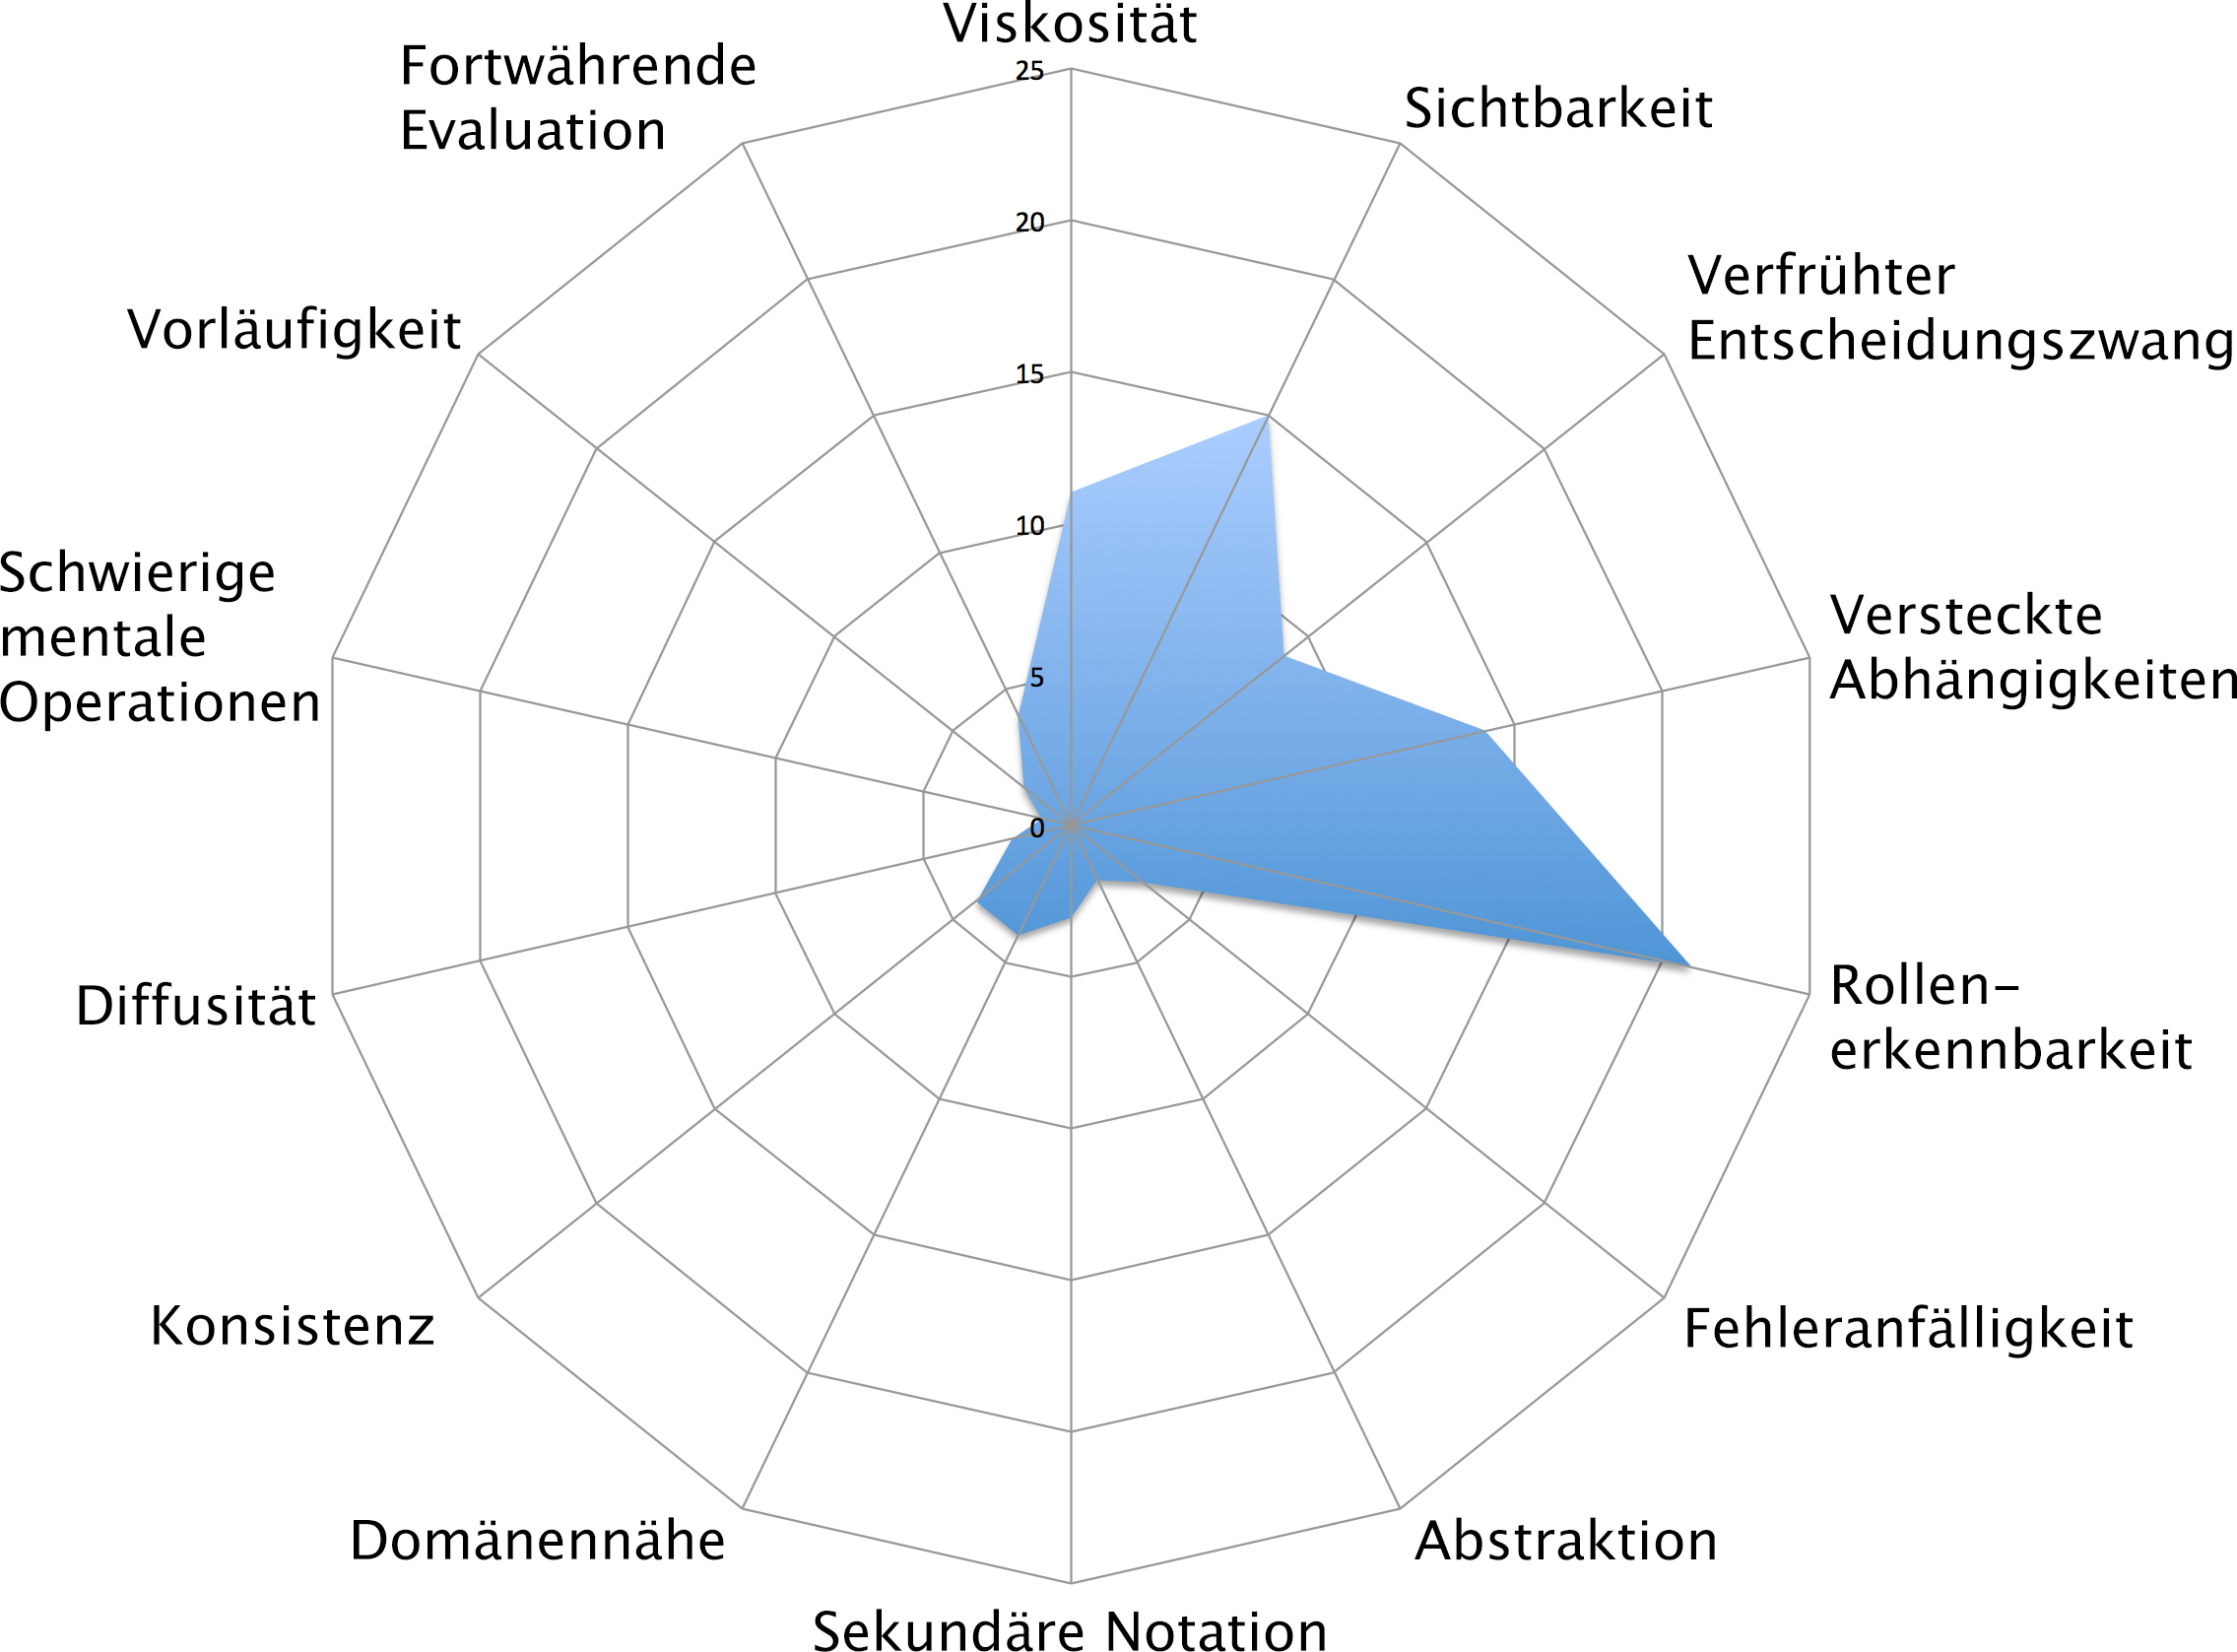
\includegraphics[width=0.7\linewidth]{Figures/cd-validierungsversuch}
  \caption[Gescheiterter Validierungsversuch mittels CDF]{Gescheiterter Versuch der Erhebung des kognitiven Profils von SeqAn mittels Cognitive Dimensions Framework}
  \label{fig:cd-validierungsversuch}
\end{figure}
\end{comment}


\subsubsection{Argumentative Validierung}

Da ich weder eine empirische (siehe \sref{sec:schwierigkeiten}), noch eine verkürzte Validierung mittels CDF vornehmen konnte, bin ich dazu gezwungen, eine argumentative Validierung durchzuführen.

Was die Auswahl der Probanden betrifft, kann ich feststellen, dass die beobachteten SeqAn-Anwender die SeqAn-Anwenderschaft für meine Forschung hinreichend repräsentieren\footnote{In der ersten Analysephase habe ich die Anwenderschaft von SeqAn charakterisiert (siehe \sref{sec:results-users}). Zu dieser gehören berufstätige, nationale und internationale Wissenschaftler aus den Bereichen Informatik, Bioinformatik und Physik. Aus diesem Grund halte ich diese Personen geeignet als Probanden für meine Forschung. Der Studentenanteil stellt keine Probleme dar, da er einen beachtlichen Teil zur bioinformatischen Arbeit beiträgt \citep{Letondal:2006dy} und damit mindestens zur zukünftigen Anwendergruppe gerechnet werden kann.}, was wichtig für valide Ergebnisse ist \citep{Clarke:2004te,Henning:2007kg}. Lediglich, wenn einzelne Usability-Probleme besser hätten verstanden werden müssen, wäre eine zielgerichtetere Auswahl der Probanden und eine langfristigere Beobachtung notwendig gewesen. Die wenigen Usability-Probleme, die ich nicht ausreichend verstanden habe, habe ich auch als solche benannt.

%Für die Validität meiner ab Seite \pageref{sec:gt} vorgestellten \gls{gt} spricht die gewissenhafte Anwendung der \gls{gtm}, denn bei der \gls{gtm} ergibt sich die Theorie ja gerade aus den Daten selbst bzw. wird in den Daten entdeckt.

Im Falle einer \gls{gtm}-basierten Forschung müsste normalerweise über das ständige Vergleichen argumentiert werden und dabei das unermüdliche Infragestellen und Überprüfen von Konzepten und Relationen gezeigt werden (siehe \sref{sec:gtm}). Dieses Vorgehen ist mir aber nicht möglich, weil es für einige meiner Konzepte und Relationen nur wenige Exemplare gibt. Außerdem sind die meisten meiner Exemplare detailarm, da sie größtenteils Ex-post-facto-Datenquellen wie der Gruppendiskussion und den Cognitive-Dimensions-Fragebögen entspringen (siehe \sref{sec:probleme-validierung}).

Meine Argumentation basiert daher auf einer Art indirekten Beweis, der nicht das ständige Vergleichen, sondern meinen auf im \sref{sec:abduktiver-blitz} vorgestellten abduktiven Blitz in den Mittelpunkt stellt. Dieser besteht darin, dass die wichtigsten Usability-Probleme auf die anwenderseitigen \code[apiua://code/-9223372036854775633]{paradigmatischen Prägungen} und den SeqAn-gestaltenden \code[apiua://code/-9223372036854775281]{Entwurfsentscheidungen} zurückzuführen sind.

Es stellt sich also die Frage, was schief gegangen sein müsste, wenn meine \gls{gt} nicht stimmen sollte. Um diese Frage zu beantworten, beleuchte ich die folgenden drei möglichen Arten von Fehlern, die mir unterlaufen sein könnten:
\begin{description}
  \item[1. Wurde ein völlig unzutreffendes Konzept bzw. Relation erkannt?] \hfill \\
  Vollkommen unzutreffende, in dieser Arbeit präsentierte Konzepte und Relationen wären den Lesern bereits in der Vorstellung der \gls{gt} aufgefallen. Für die Überprüfung stehen sowohl die angegebenen, mit einem \raisebox{-0.3ex}{
\includegraphics[height=2.2ex]{Figures/openaccess.pdf}}-Symbol versehenen Exemplare, die zu den Konzepten gehörigen Memos und die insbesondere bei den vornehmlich technisch-deduktiven Konzepten angegebene Literatur zur Verfügung.

  \begin{description}
    \item[Beispiel 1] \hfill \\
    Nehmen wir als Beispiel das folgende Exemplar, welches die Antwort eines Probanden\citepurl{apiua://survey/cd/2013-09-19T11:51:16.616+02:00} auf die Frage nach der \glslink{cd}{kognitiven Dimension} \textit{Hard Mental Operations} (siehe \aref{app:cdf-questions}) war.
  
    \textbf{Frage:} ``Do some things in SeqAn seem especially complex or difficult to work out in your head (e.g. when combining several things)? What are they?''\\
    \textbf{Antwort:} ``Yes, remembering all the templates and variants of types and templates and trying to figure out what is the difference between say Dna5 and Dna5String.''\citepurl{apiua://survey/cd/2013-09-19T11:51:16.616+02:00/hardMentalOperations}
    
    Bei naiver Lesart könnte man zu dem Schluss kommen, dass die Kernaussage des Probanden darin besteht, dass die Vielzahl an Templates und Typvarianten deren Einprägen verhindert. Ein mögliches Konzept hieße also \code{Template-/Typ-Variantenübermaß} oder etwas deskriptiver \code{Nicht einprägsames Template-/Typ-Variantenübermaß}.
    
    Wendet man hingegen die \textit{wortgenaue Analyse} nach \cite{charmaz2006constructing} an, ergibt sich folgende stichpunktartige Paraphrase:
    \begin{itemize}
    \itemsep1pt\parskip0pt\parsep0pt
    \item remembering complicated
      \begin{itemize}
        \item many templates
        \item many variants of types
        \item many variants of templates
      \end{itemize}
      \item difference unclear
      \begin{itemize}
        \item e.g. Dna5 and Dna5String
      \end{itemize}
    \end{itemize}
    
    Schaut man sich darüber hinaus die übrigens Antworten des Teilnehmers an (``typing / templates seem to be extremely messy''\citepurl{https://github.com/bkahlert/seqan-research/blob/master/raw/workshop13/workshop2013-data-20130926/cd/2013-09-19T11-51-16.61646000\%2B0200.xml\#L21}, ``you need to take care of types, type casting, [\ldots] etc. ``99\% of the cases [\ldots] will not even compile''\citepurl{apiua://survey/cd/2013-09-19T11:51:16.616+02:00/errorProneness}, ``[requires] me to spend time on getting type casting right''\citepurl{apiua://survey/cd/2013-09-19T11:51:16.616+02:00/provisionality}, \ldots) erkennt man, dass es gar nicht um das Einprägen von Templates oder Typvarianten geht. Vielmehr wird deutlich, dass der Proband jede gestellte Frage nutzt, um seinen Verdruss über die Art zum Ausdruck bringt, wie schwer der Umgang mit Typen in SeqAn ist.
    
    Das in meinen Augen korrekte Konzept lautet also \code{apiua://code/-9223372036854775352} (siehe Seite \pageref{sec:typing}). Dieses Konzept befasst sich mit den Problemen, die Anwender bei der Deklaration von Typen, bei Type-Castings, beim Setzen von Parametern von Klassen- und Funktionstemplates und bei der Berechnung von Rückgabetypen mittels Metafunktionen haben.
    
    Der zweite Teil der Aussage des Probanden bezieht sich auf die unklare Unterscheidbarkeit von der \texttt{String}-Klasse und ihren Spezialisierungen, was ich als \code{apiua://code/-9223372036854775335} bezeichne\footnote{In SeqAn dienen die \texttt{Dna}-Varianten als Spezialisierung der \texttt{String}-Klasse, was ich fachlich für inkorrekt halte. Tatsächlich müsste es \texttt{Nucleotide}-Varianten geben, die String spezialisieren. Folglich müsste \mintinline{cpp}{Dna} als \mintinline{cpp}{typedef String<Nucleotide>} definiert sein.}, aber wegen der ohnehin schon vielen wichtigen Erkenntnisse nicht weiter verfolgt habe.
    
    \item[Beispiel 2] \hfill \\
    Auf die Frage zur CD \textit{Viskosität}\footnote{Der Fragebogen wurde sowohl auf Deutsch wie auch auf Englisch angeboten. Daher gebe ich die Übersetzung an, die der Proband mit großer Wahrscheinlich auch gelesen hat.} (siehe \aref{app:cdf-questions}) antworte ein anderer Proband\citepurl{apiua://survey/cd/2013-09-18T17:50:13.425+02:00} wie folgt:
  
    \textbf{Frage:} ``Wenn du Änderungen am Code durchführst, welche fallen dir am schwersten/aufwendigsten? Warum?''\\
    \textbf{Antwort:} ``Wenn es wenig Beispiele gibt bzw. die Funktionalitaet mancher Konstrukte zu ergruenden ist''\citepurl{apiua://survey/cd/2013-09-18T17:50:13.425+02:00/viscosity}
    
    Bei dieser ziemlich knappen Antwort könnte man glauben, dass der Proband hinterfragt, was manche ``Konstrukte'' genau tun. Das Konzept könnte also \code{Unklare Konstrukt-Funktionalität} heißen.
    
    Aber auch hier wäre die naive Lesart unpassend und die Betrachtung der übrigen Antworten desselben Probanden anzuraten:
    \begin{itemize}
      \item Antwort auf die Frage zur CD \textit{Schwierige mentale Operationen}: ``Wenn viele Konzepte und Konstrukte ineinandergreifen ist es teils die Verwendung teils schwer. Klar ;)''\citepurl{apiua://survey/cd/2013-09-18T17:50:13.425+02:00/hardMentalOperations}
      \item Antwort auf die Frage zur CD \textit{Fortschreitende Evaluation}: ``Wenn man lange nach bestimmten Funktionen sucht bzw. lange braucht deren Verwendung zu verstehen ist der Fortschritt manchmal schwer zu ueberblicken. Im Prinzip aber ja.''\citepurl{apiua://survey/cd/2013-09-18T17:50:13.425+02:00/progressiveEvaluation} 
    \end{itemize}
    
    Bei Betrachtung dieser beiden weiteren Antworten wird deutlich, dass es nicht um die ``Funktionalität'' von ``Konstrukten'', sondern um deren ``Verwendung'' geht. In Verbindung mit dem gleichzeitigen Auftreten der Begriffe ``Konzepte'', ``Konstrukte'' und ``Funktionen'' schließe ich, dass es neben den \code[apiua://code/-9223372036854775581]{fehlenden Anwendungsbeispielen} im Kern um das Usability-Problem \code{apiua://code/-9223372036854775405} (siehe Seite \pageref{sec:typing}) geht. Dieses Konzept befasst sich mit der anwenderseitigen Frage, wie Funktionen verwendet werden. Es handelt sich dabei um ein Elternkonzept des schon genannten \code{apiua://code/-9223372036854775352}-Konzepts (vgl. \sref{sec:gtm-modellierung}: ``Modellierung der Ergebnisse'').

    \item[Beispiel 3] \hfill \\
    Wenn man sich noch einmal Beispiel 2 ansieht und sich fragt, welche Relationen in der Antwort ``Wenn es wenig Beispiele gibt bzw. die Funktionalitaet mancher Konstrukte zu ergruenden ist''\citepurl{apiua://survey/cd/2013-09-18T17:50:13.425+02:00/viscosity}  auf die Viskositätsfrage ``Wenn du Änderungen am Code durchführst, welche fallen dir am schwersten/aufwendigsten? Warum?'' stecken, sieht man die folgende Relation leicht ein: \rel[\apiuaLink{apiua://relation/7omanqrfcmabqmcmk1nftt781rbf7ovo}{verlangsamen}]{\code[apiua://code/-9223372036854775581]{Fehlende Anwendungsbeispiele}}{\code{apiua://code/-9223372036854775455}}.
    
    Wäre man dem Irrtum erlegen, der Proband spräche von der ``Funktionalität mancher Konstrukte'', hieße eine weitere, inkorrekte Relation \rel[verlangsamt]{\code{Unklare Konstrukt-Funktionalität}}{\code{apiua://code/-9223372036854775455}}. Tatsächlich verbirgt sich aber die folgende Relation in der Antwort: \rel[\apiuaLink{apiua://relation/kaj841regkeu1so0ut5neslol9vfn837}{verlangsamt}]{\code{apiua://code/-9223372036854775405}}{\code{apiua://code/-9223372036854775455}}.
    
    Nach mehreren Monaten der Datenanalyse habe ich eine gewisse theoretische Sensibilität erlangt, die mir auch dabei half, Begriffe wie ``Konstrukte'', ``Konzepte' und ``Idiome'' zu deuten. Aus dem breiten Kontext wird deutlich, dass diese Begrifflichkeiten auf den für die beobachteten \code[apiua://code/-9223372036854775494]{paradigmatischen Prägungen} untypischen Entwurf von SeqAn abzielen. Dieser ist geprägt, durch Elemente wie Metafunktionen, Tags und Interface-Funktionen, welche ich zusammengefasst als \code{apiua://code/-9223372036854775413} bezeichne (siehe Seite \pageref{sec:gt-let}). Daraus ergibt sich die folgende weitere Relation: \rel[\apiuaLink{apiua://relation/thq387lsd79dmprfs03flmkdtu23uh4b}{erschweren}]{\code{apiua://code/-9223372036854775413}}{\code{apiua://code/-9223372036854775405}}.
    
    Ohne diese theoretische Sensibilität und ohne Betrachtung anderer Datenpunkte des gleichen Probanden, wäre man Gefahr gelaufen, den Begriff ``Konstrukt'' als Schleifenkonstrukt, Funktionsbezeichner oder ähnliches fehlzudeuten. Schleifenkonstrukte sind in der Tat eine mögliche, alternative Deutung, denn in SeqAn werden in Schleifen Iteratoren verwendet. Da Iteratoren wiederum  mit Hilfe von Metafunktionen konstruiert werden, werden auch die Schleifenkonstrukte schwerer verständlich. Derartige Fehlinterpretationen können jedoch weitgehend ausgeschlossen werden, denn häufig benennen Probanden Iteratoren auch als solche\citepurl{apiua://survey/cd/2013-09-18T17:45:54.889+02:00/roleExpressiveness}\citepurl{apiua://groupDiscussion/workshop\%2712+-+Interview+Gruppendiskussion+\%282012-09-06T13-01-28\%2B0200\%29.html/li/4}. Im konkreten Beispiel kommt hinzu, dass der Proband bereits seit vier Jahren SeqAn nutzt\citepurl{https://github.com/bkahlert/seqan-research/blob/master/raw/workshop13/workshop2013-data-20130926/cd/2013-09-18T17-50-13.42530400\%2B0200.xml\#L6} und Iteratoren zu den Pflicht-Tutorials eines jeden SeqAn-Anfängers gehören\citepurl{http://seqan.readthedocs.org/en/master/Tutorial/Iterators.html}.
  \end{description}
  
  \item[2. Wurde ein Konzept bzw. Relation weit unterschätzt?] \hfill \\
  Die Wahrscheinlichkeit einer Unterschätzung wurde durch die weiter oben beschriebene Triangulation verringert. Es ist anzunehmen, dass wichtige Konzepte bzw. Relationen in meiner breit angelegten Datenerhebung (siehe \sref{sec:phase2}) häufiger oder intensiver vertreten und damit weniger leicht zu unterschätzen sind.
  
  Außerdem habe ich die Daten sehr genau (siehe obige Beispiele) analysiert. Dies verringerte ebenfalls die Wahrscheinlichkeit, dass ich wichtige Konzepte bzw. Relationen übersehen habe.
  
  Des Weiteren erhebe ich keinen Anspruch auf Vollständigkeit. Es liegt in der Natur der Sache, dass ein anderer Forscher Problemarten gefunden hätte, für die ich blind war oder denen ich weniger Aufmerksamkeit zukommen ließ. Zum Beispiel habe ich dem Usability-Problem \code[apiua://code/-9223372036854775512]{Fehleranfälliger Gebrauch von \texttt{const}} relativ früh wenig Aufmerksamkeit beigemessen, weil die ersten Phänomene mir klar zeigten, dass es sich um ein reines C\texttt{++}-Anfängerproblem handelte. Möglicherweise wäre ich eines besseren belehrt worden, hätte ich dieses Konzept intensiver beforscht.
  
  Ähnlich verhält es sich mit der Relation \rel[\apiuaLink{apiua://relation/aknb7upadsapb65at08319ipqcq3oink}{erleichtern}]{\code{apiua://code/-9223372036854775271}}{\code{apiua://code/-9223372036854775262}}, die eine Folge der im \sref{sec:phase1} beschriebenen Usability-Verbesserung im Rahmen der ersten Beseitigung grober Usability-Probleme darstellt und darüber hinaus bereits im \sref{sec:phase1-validierung} validiert wurde.
  
  
  \item[3. Wurde ein Konzept bzw. Relation weit überschätzt?] \hfill \\
  Diese Frage kann mit der Tatsache beantwortet werden, dass ich die SeqAn-Entwickler zur Umsetzung vieler der auf meinen Ergebnissen basierenden Usability-Verbesserungsmaßnahmen bewegen konnte.
  
  In \sref{sec:seqan-api-usability-vorschlaege} habe ich Verbesserungsmöglichkeiten vorgeschlagen. Den erwarteten Einfluss auf den  Grad der Verbesserung habe ich wiederum auf Grundlage meiner Analyseergebnisse geschätzt. Von den vier wertvollsten Maßnahmen, wurden drei Maßnahmen umgesetzt --- nämlich (1) die Verwendung von KNIME als API-Endanwender-Werkzeug, (2) den Umbau von SeqAn von einem Framework zu einer Library und (3) die Überarbeitung der SeqAn-Dokumentation (siehe \sref{sec:seqan-api-usability-verbesserung}). Abgesehen von der technischen Neuentwicklung der Dokumentation, wurde ein beachtlicher Teil der Arbeit durch die SeqAn-Entwickler gestemmt. Dies zeigt, dass die SeqAn-Entwickler meine Einschätzung der wichtigen gefundenen Konzepte und Relationen teilen.
  
  Interessanter ist die vierte wichtige Maßnahme, die in der Angleichung an die STL besteht: Ich habe das für die Umsetzung der Maßnahme notwendige CRTP einigen SeqAn-Entwicklern zu einer Zeit präsentiert, in der ich noch in dem Glauben war, SeqAns Anwender würden eine streng objektorientierte Library erwarten. Dies entsprach zum Einen nicht den Tatsachen, denn ein großer Teil erwartete lediglich eine STL-konforme Softwarebibliothek (siehe \code{apiua://code/-9223372036854775494}, Seite \pageref{sec:paradigmatische-pragung}). Zum Anderen stieß ich mit diesem Vorschlag auf Ablehnung, denn mit Ausnahme des übrigen SeqAn-Entwicklers Andreas Gogol-Döring, der begeistert von meinem Vorschlag war \citep[][siehe \sref{sec:verbesserung-crtp}]{GogolDoring:5iYhf2VJ}, scheuten die damaligen SeqAn-Entwickler verständlicherweise die damit verbundenen Kosten, welche sie zusätzlich zu tragen hätten. Aus zeitlichen Gründen kam ich nicht mehr dazu, dem SeqAn-Team meinen neuen Erkenntnisstand mitzuteilen. An dem Nutzen dieser Maßnahme besteht indes kein Zweifel, denn die teils hitzigen Wortmeldungen in den unterschiedlichen Datenquellen (``Vergewaltigung der OO-Programmierung''\citepurl{apiua://survey/2011-09-14-T15:23:17.211+02:00}, ``[It's] not clear why you have to go through all this pain''\citepurl{apiua://groupDiscussion/workshop\%2712+-+Interview+Gruppendiskussion+\%282012-09-06T13-01-28\%2B0200\%29.html/li/14}) sprechen eine eindeutige Sprache (siehe \code{apiua://code/-9223372036854775633}, Seite \pageref{sec:stl-inconsistencies}).  
  
  Nicht alle Usability-Probleme wurden gelöst, da nicht alle vorgeschlagenen Maßnahmen umgesetzt wurden:
  \begin{itemize}
    \item Konzepte, die ich nicht hinreichend gut verstanden habe (z.B. \code{apiua://code/-9223372036854775116}, \code{apiua://code/-9223372036854774846} und \code{apiua://code/-9223372036854774861}, siehe \sref{sec:Inkonsistenzbeseitigung}), wurden auch als solche benannt und werden im Ausblick thematisiert. Hier besteht also keine Gefahr einer Überschätzung.
    \item Die übrigen Konzepte und Relationen wurden entweder nur durch einen Teil der SeqAn-Entwickler oder von keinem der SeqAn-Entwickler ähnlich eingeschätzt. Zu Ersteren gehört die \code{apiua://code/-9223372036854775615}. Zu Letzteren gehört die \code{apiua://code/-9223372036854774861}. An dieser Stelle der Argumentation kann ich lediglich auf die Plausibilität meiner ab Seite \pageref{sec:gt} dargestellten \gls{gt} und auf meine weiter oben angesprochene theoretische Sensibilität verweisen. 
  \end{itemize}
\end{description}


%Alle wichtigen Verfahrensschritte wurden von mir ausführlich beschrieben und Ergebnisse mit Hilfe von Literatur und der Analyse unterschiedlicher Datenquellen trianguliert. Das Gesamtbild meiner Theorie bewerte ich als schlüssig.

Da nun die Frage nach der Validität meiner in dieser Arbeit präsentierten \gls{gt} geklärt ist, gilt es noch zu untersuchen, ob meine vorgeschlagenen Maßnahmen die entsprechenden Usability-Probleme korrekt adressieren und ob die umgesetzten Maßnahmen auch tatsächlich zu einer Usability-Verbesserung beigetragen haben.

Die von mir formulierten Maßnahmen betreffen weitgehend eine disjunkte Menge von Usability-Problemen. Bei einigen Usability-Problemen (Maßnahmen \textit{Frameworkumbau}, \textit{Fail-Fast}, \textit{Kollaborationsplattform} und \textit{Werkzeugunterstützung}) lag die Lösung auf der Hand. War dies nicht der Fall, habe ich argumentiert, an welcher Stelle die Maßnahme ansetzt und in welchem Umfang welche Usability-Probleme damit gelöst werden (z.B. \textit{Maßnahme STL-Angleichung}).

Ob die praktische Ausgestaltung einer Maßnahme tatsächlich den gewünschten Effekt hatte, diskutiere ich im Folgenden:
\begin{itemize}
  \item Die \textit{STL-Angleichung} wurde leider noch nicht umgesetzt. Insbesondere die Analyseergebnisse der Gruppendiskussion sind  bzgl. der Lösung derart eindeutig, dass kein Zweifel über die inhaltliche Eignung des CRTP besteht. Darüber hinaus wurde das CRTP bereits in einigen Boost-Libraries und der Microsoft Active Template Library eingesetzt, was technische Bedenken bzgl. der Umsetzbarkeit weitgehend ausräumt.
  \item Das gleiche gilt für die, durch die \code{apiua://code/-9223372036854775281} \code{apiua://code/-9223372036854774838} verursachten \code{apiua://code/-9223372036854775117}, welche durch die Maßnahme \textit{Inkonsistenzbeseitigung} behoben werden sollen.
  \item Ebenso eindeutig sind die Gruppendiskussionsergebnisse in Bezug auf die Maßnahme \textit{Shortcuts}, welche die, durch die gleichnamige \code{apiua://code/-9223372036854775281} verursachten Probleme \code{apiua://code/-9223372036854774861} und \code{apiua://code/-9223372036854774860} beheben soll.
  \item Die Entwicklung einer \textit{Wrapper-API} durch die Integration von SeqAn-Knoten in die Workflow-Engine KNIME muss auf verschiedene Weise argumentiert werden.
  \begin{enumerate}
    \item Die Eignung von grafischen Entwicklungsumgebungen für die Verbesserung der API-Usability für API-Endanwender ist vielfach gezeigt worden \citep{Ko:2011el}.
    \item Da die SeqAn-Knoten direkt in den KNIME-Mechanismus zum Beziehen von Dritthersteller-Knoten integriert wurden, kommt es an dieser Stelle zu keiner Kompromittierung der Usability.
    \item Allerdings kommt es durch die Einbindung von Kommandozeilenprogrammen in KNIME zu einem Paradigmenwechsel. KNIME transferiert zwischen den datenverarbeitenden Knoten Daten in Form von Tabellen. SeqAn-Anwendungen verwenden für die Ein- und Ausgabe hingegen Dateien. Um eine ideale Integration zwischen gewöhnlichen KNIME- und SeqAn-Knoten zu ermöglichen, wurden Konverterknoten implementiert, welche Tabellen zu Dateien und anders herum konvertieren können. Ob und welche Anwendungsschwierigkeiten sich daraus ergeben, habe ich nicht evaluiert.
    \item Nicht zuletzt hängt die Usability der Wrapper-API von der Usability von KNIME selbst ab, das ebenfalls nicht Gegenstand einer Evaluation war. Die weite Verbreitung von KNIME lässt zumindest darauf schließen, dass es sich hierbei nicht um ein K.O.-Kriterium\footnote{Wissenschaftlich korrekt ausgedrückt, handelt es sich hierbei um die vierte boolesche Eigenschaft \textit{Markteinfluss}, die von \cite{Sarodnick:2006vc} zur Bewertung der Fatalität eines Usability-Problems herangezogen wird. Diese Eigenschaft ergänzt die ursprünglichen drei von \cite{Nielsen:1994tx} formulierten Eigenschaften.} handelt.
  \end{enumerate}
  \item Die Validierung der Maßnahme \textit{Intransparenzbeseitigung} kann wegen unzureichender empirischer Erkenntnisse nicht geleistet werden. Dazu muss das Usability-Problem \code[apiua://code/-9223372036854775057]{versteckte Parameterübergabe} besser erforscht werden.
  \item Die Dokumentation wurde umfangreich verbessert (siehe \sref{sec:improve-dox}):
  \begin{enumerate}
    \item Die Umstellung des Dokumentationssystems wurde von den SeqAn-Entwicklern als wichtig und sinnvoll erachtet, was sich auch an ihrer mehrwöchigen, inhaltlichen Mithilfe zeigte.
    \item Auch der Entwicklermodus wurde positiv von den SeqAn-Entwicklern angenommen. Dieser wird regelmäßig genutzt, um Dokumentationseinträge stärker zu verlinken.
    \item Die positiven Auswirkungen eines Gesamtüberblicks und von Beispielen sind bereits vielfach in der Literatur beschrieben worden (siehe \sref{sec:forschung-einzelne-ergebnisse}). Es ist daher naheliegend, dass der neu geschaffene Gesamtüberblick und die ergänzten bzw. korrigierten Beispiele (siehe jeweils \sref{sec:improve-dox}) zu einer signifikante Verbesserung der API-Usability beigetragen haben.
    \item Die Verbesserung der Suchfunktion ist eine direkte Konsequenz aus den von den Anwendern geäußerten Kritikpunkten. Die Unterstützung von Aliassen und einer gewichteten Suche (siehe  \sref{sec:improve-dox}) lassen den Schluss auf eine Usability-Verbesserung zu.
    \item \code{apiua://code/-9223372036854775413} werden in keiner mir bekannten C\texttt{++}-Library, die auf Templatemetaprogrammierung basiert, explizit zu Dokumentationszwecken eingesetzt. Dafür gibt es zwei mögliche Gründe.
    \begin{itemize}
      \item Entweder richten sich derartige Libraries an fortgeschrittene Entwickler\footnote{Typische Vertreter sind die Boost-Libraries wie BCCL (\url{http://www.boost.org/doc/libs/1_58_0/libs/concept_check/concept_check.htm}) oder CRC(\url{http://www.boost.org/doc/libs/1_58_0/libs/crc/}).}, was den Erklärungsbedarf anspruchsvoller Sprachentitätstypen deutlich verringert.
      \item Oder aber entsprechende Libraries verbergen für Anfänger ungeeignete Sprachentitätstypen beispielsweise durch den Einsatz von CRTP\footnote{Zu den bekanntesten Vertretern gehört die Microsoft Active Template Library (\url{https://msdn.microsoft.com/en-us/library/4e07a759.aspx}).}.
    \end{itemize}
    SeqAn wendet sich sowohl an API-Anwendern als auch an API-Endanwender und damit auch an weniger erfahrene Entwickler. Meine Forschungsergebnisse haben gezeigt, dass das fehlende Verständnis neuartiger Sprachentitätstypen wie Interface-Metafunktionen zu Usability-Problemen führt. Daher besteht für mich kein Zweifel daran, dass die explizite Einführung dieser Sprachentitätstypen zu einer Usability-Verbesserung beiträgt.
  \end{enumerate}
  \item Den positiven Effekt von Verbesserungen aus der ersten Beseitigung grober Usability-Probleme habe ich --- insbesondere für die überarbeiteten Installationsanleitungen und Tutorials --- bereits im \sref{sec:phase1-validierung} argumentativ und empirisch gezeigt.
\end{itemize}

\bigskip

Es ist davon auszugehen, dass der Umfang der Überarbeitung der SeqAn-API eine erneute Validierung sinnvoll macht. Es ist nicht auszuschließen, dass das Zusammenspiel der Maßnahmen zu neuen emergenten Usability-Problemen geführt hat. Diese Vermutung wird durch die Aussage von \cite{Stylos:2009ts} gestützt, dass bereits kleine API-Anpassungen große Auswirkungen auf die Usability haben können.





\subsection{Verallgemeinerbarkeit}

\begin{comment}
Fertigstellungskriterien nach \citep{glaser2005grounded}: vin Salinger kopiert
\begin{itemize}
  \item Der entwickelte ``konzeptionelle Rahmen'' bildet eine ``systematische Theorie'', also etwas fokussiert und strukturiert Beschreibendes, Erklärendes oder Vorhersagendes,
  \item was eine ``hinreichend präzise'' Antwort auf die ursprüngliche, bzw. sich weiterentwickelte Frage liefert
  \item und von anderen Forschern, die verwandte Gebiete untersuchen, verwendet werden kann.
\end{itemize}
\end{comment}

Es lassen sich sowohl methodische, softwaretechnische und Usability-Problem-bezogene Erkenntnisse verallgemeinern.


\subsubsection{Methodische Erkenntnisse}

Meine Erkenntnisse und die Generizität meiner Methode belegen, dass sich meine Forschungsmethode sehr gut für die Erforschung \textit{un}typischer APIs eignet. Die Generizität ergibt sich einerseits aus der breit angelegten Datenerhebung, und andererseits aus dem extrem offenen Forschungsansatz der \gls{gtm}.

Insbesondere die Programmierschritte-Datenerhebung eignet sich auch unter Rahmenbedingungen, bei denen es nur wenige Möglichkeiten zur Datenerhebung gibt, weil besonders viele Daten automatisiert erhoben werden und praktisch keine Beeinflussung der Probanden stattfindet (siehe \sref{sec:phase2-fazit}). Aus Zeitgründen konnte ich leider nur wenige Erkenntnissen aus dieser Datenquelle ziehen, weshalb ich letztere Aussage kaum empirisch belegen kann.

Die sich aus meiner Forschungsmethode ergebende Erkenntnisfülle hat aber auch eben diesen Preis: den hohen Zeitaufwand. Durch die Erhebung sowohl subjektiver, als auch objektiver Daten, verbunden mit der leichtgewichtigen \acrshort{he} und der schwergewichtigen \gls{gtm}, kann der Forscher nicht mit schnellen Ergebnissen rechnen. Außerdem benötigt er für die Programmierfortschritte-Daten ein geeignetes Datenanalysewerkzeug, wie der im \sref{sec:apiua} vorgestellte \gls{apiua}.

APIUA ist aktuell zwar explizit auf meine Forschung zugeschnitten, erlaubt durch seine komponentenbasierte Architektur aber eine einfache Erweiterung um die Unterstützung neuer Datenformate. Jedoch kann ich nicht verschweigen, dass der praktischen Nutzung noch die relativ geringe Stabilität im Wege steht. Der für die Datenerhebung notwendige Webclient kann ohne Anpassungen für andere Forschungsvorhaben eingesetzt werden. Der lokal arbeitende Client hingegen muss in den lokalen Build-Prozess integriert werden, was im Falle des von SeqAn eingesetzten CMake problemlos möglich war, anderenfalls aber aufwändiger sein könnte.

Die Eignung meiner Forschungsmethode für meine durchgeführte Forschung beweisen meine Ergebnisse. Die Eignung für andere Forschungsvorhaben habe ich soeben argumentiert. Ob dies tatsächlich zutrifft, müsste durch die Durchführung einer Vielzahl unterschiedlicher Forschungsvorhaben mit meiner Methode belegt werden. Zumindest kann ich zu meiner Verteidigung ins Feld führen, dass der empirische Beleg von keiner der in der Literatur beschriebenen komplexen API-Usability-Evaluationsmethoden erbracht wurde (siehe \sref{sec:datenerhebung}).

Die folgenden zwei Unterabschnitte sind gegliedert in methodische und problembezogene Erkenntnisse. Methodische Erkenntnisse umfassen Einsichten, die sich auf den Entwicklungsprozess von APIs beziehen. Problembezogene Erkenntnisse hingegen behandeln die Frage, mit welchen Usability-Problemen API-Entwickler bei der Entwicklung rechnen müssen. 


\subsubsection{Softwaretechnische Erkenntnisse}

\begin{enumerate}
  \item Die Entwicklung von SeqAn hat gezeigt, dass nicht-empirische Entwurfsentscheidungen nicht zwingend zum Erreichen der erdachten Ziele führen. Ist es \textit{tatsächlich} so, dass ein Entwurfsziel primär und die anderen sekundär sind, deuten meine Forschungsergebnisse darauf hin, dass die sekundären Entwurfsentscheidungen nicht gründlich genug umgesetzt werden, im Zweifel unterliegen und zu schweren bis katastrophalen Problemen führen können.
  
  Im Falle von SeqAn stellt Performance das primäre Ziel und Usability de facto das sekundäre Ziel dar (siehe \sref{sec:gt}).
  
  \item Ein Prioritätenwechsel, wie dies bei SeqAn die neue Betonung der Usability war (siehe \sref{sec:gt-urursache}), zeigt, dass für tolerierbar gehaltene oder gar nicht wahrgenommene Usability-Probleme plötzlich eine große Wichtigkeit bekommen können. Die nachträgliche Diagnose und Behebung solcher Usability-Probleme kann sehr aufwändig sein. Meine Arbeitszeit erstreckte sich über knapp vier Jahre. Hinzu kamen die unzähligen Personenmonate, die meine SeqAn-Kollegen aufbrachten. %Dieser enorme Kostenaufwand ist unter dem Namen \textit{Rule of Ten} bekannt \citep[u.a.][]{clark1991product,boehm1981software}.

  \item Bei der Entwicklung eines Produkts ist ein gründliches und gemeinsames Verständnis über die (zukünftigen) Anwender existenziell wichtig. Dies ist bereits in der Literatur bekannt \citep[u.a.][]{Clarke:2004te,Henning:2007kg}.
  
  Im SeqAn-Team lag nur ein unzureichendes Verständnis von den Anwendern vor, worin eine der Hauptursachen für die entdeckten Probleme bestand. Des Weiteren gab es Uneinigkeit in der Frage, ob Entwickler mit wenig Programmiererfahrung zur Anwenderschaft gehören. Dies führte dazu, dass bekannte Anwendungsschwierigkeiten nicht als zu behebende bzw. zu vermeidende Usability-Probleme eingestuft wurden. Meine Beobachtungen bestätigen also die Notwendigkeit, eine fundierte und gemeine Vorstellung von den Zielgruppen zu haben, wenn Usability-Probleme vermieden werden sollen.
\end{enumerate}


\subsubsection{Usability-Problem-bezogene Erkenntnisse}

Bis auf die beiden weitgehend SeqAn- bzw. Gogol-Döring-spezifischen Probleme \code{apiua://code/-9223372036854774829} und \code{apiua://code/-9223372036854774860}, lassen sich die übrigen von mir entdeckten Probleme unterschiedlich stark verallgemeinern. Die Gründe der Verallgemeinerung können den Usability-Problem-Beschreibungen im \sref{sec:gt} entnommen werden.

Da ich mich mit einer C\texttt{++}-basierten Library beschäftigt habe, gelten die im Folgenden genannten Usability-Probleme möglicherweise nicht bei Programmiersprachen, die nicht über bestimmte Sprachfeatures, wie die Überladbarkeit von Operatoren, verfügen. Andere Probleme lassen sich hingegen leicht auf die eigene Programmiersprache übertragen. So würde das Problem \code{apiua://code/-9223372036854775633} im Falle von Java beispielsweise \textit{Inkonsistenzen bzgl. JDK} lauten, denn der Kern dieses Problems ist nicht die STL, sondern die Enttäuschung der sich aus der \code[apiua://code/-9223372036854775494]{paradigmatischen Prägung} ergebenden Erwartungen.

\begin{description}\raggedright
  \item[Allgemeine Probleme] \hfill \\ Probleme, die in jeder API auftreten können.
  \begin{description}\raggedright
    \item[\codebullet{apiua://code/-9223372036854774915}] \codetext{apiua://code/-9223372036854774915} \\
    \code{apiua://code/-9223372036854775623}, \code{apiua://code/-9223372036854775567}, \code{apiua://code/-9223372036854774861}, \code{apiua://code/-9223372036854775533}
    
    \item[\codebullet{apiua://code/-9223372036854775404}] \codetext{apiua://code/-9223372036854775404} \\
    \code{apiua://code/-9223372036854775581}
    
    \item[\codebullet{apiua://code/-9223372036854774914}] \codetext{apiua://code/-9223372036854774914} \\
    \code{apiua://code/-9223372036854775615}
  \end{description}
  
  \item[Probleme der Templatemetaprogrammierung] \hfill \\ Probleme, die in APIs auftreten können, die Templatemetaprogrammierung einsetzen.
  \begin{description}
    \item[Inhärente Probleme] \hfill \\ Probleme, mit deren Auftreten bei der Verwendung von Templatemetaprogrammierung gerechnet werden muss und die proaktiv ausgeschlossen werden müssen.
    \begin{description}
      \item[\codebullet{apiua://code/-9223372036854774915}] \codetext{apiua://code/-9223372036854774915} \\
      \code{apiua://code/-9223372036854775080}, \code{apiua://code/-9223372036854775633}, \code{apiua://code/-9223372036854775413}, \code{apiua://code/-9223372036854775279}, \code{apiua://code/-9223372036854775405}
    
      \item[\codebullet{apiua://code/-9223372036854775404}] \codetext{apiua://code/-9223372036854775404} \\
      \code{apiua://code/-9223372036854775280}, \code{apiua://code/-9223372036854775544}
    
      \item[\codebullet{apiua://code/-9223372036854774914}] \codetext{apiua://code/-9223372036854774914} \\
      \code{apiua://code/-9223372036854775100}
  
      \item[\codebullet{apiua://code/-9223372036854775396}] \codetext{apiua://code/-9223372036854775396} \\
      \code{apiua://code/-9223372036854775148}
    \end{description}
  
    \item[Mögliche Probleme] \hfill \\ Probleme, die mit einer gewissen Wahrscheinlichkeit --- insbesondere im Hinblick auf generische Programmierung --- auftreten.
    \begin{description}
      \item[\codebullet{apiua://code/-9223372036854774915}] \codetext{apiua://code/-9223372036854774915} \\
      \code{apiua://code/-9223372036854775116}, \code{apiua://code/-9223372036854774846}, \code{apiua://code/-9223372036854775057}
    
      \item[\codebullet{apiua://code/-9223372036854775404}] \codetext{apiua://code/-9223372036854775404} \\
      \code{apiua://code/-9223372036854775572}, \code{apiua://code/-9223372036854775577}, \code{apiua://code/-9223372036854775504}, didaktische Lernressourcen wie \code{apiua://code/-9223372036854775271}
    \end{description}
  \end{description}
\end{description}

\bigskip

Für den Verallgemeinerungsgrad der oben genannten Usability-Probleme habe ich auch die zu erwartenden Fatalitäten der Probleme betrachtet. So stellt ein \code{apiua://code/-9223372036854775572} wahrscheinlich bei jeder API ein Usability-Problem dar. Jedoch ist es bei generischer Programmierung besonders schwerwiegend, weshalb ich es entsprechend eingeordnet habe.


\begin{comment}
\subsubsection{Bedrohungen der Validität}

Ich habe die \gls{gtm} während meiner Forschung und der Entwicklung meines qualitativen Datenanalysewerkzeugs erlernt. Auch wenn ich davon ausgehe, dass dieses Wechselspiel zu einer tieferen Erkenntnis geführt hat, kann ich nicht ausschließen, dass meine spezielle Datenerhebung zu einem windschiefen, atypischen \gls{gtm}-Verständnis geführt hat.

Meine mangelhaften Bioinformatik-Kenntnisse empfand ich nur selten als hinderlich, zumal ich mich bei Unklarheiten an meine Arbeitskollegen aus der AG Bioinformatik gewandt habe. Dennoch besteht die Gefahr, dass ich für fachlich bedingte Usability-Probleme, deren Ursachen und Folgen blind war.

Die Verwendung selbst entwickelter Interferenzregeln innerhalb meines Datenanalysewerkzeugs haben meine \gls{gtm}-Arbeitsweise beeinflusst. Nach meiner Einschätzung positiv. Aber auch hier kann ich nicht ausschließen, dass mögliche Erkenntnisse durch die Funktionen verdeckt wurden.

Es stellt sich die Frage, ob meine qualitative Betrachtung der SeqAn-Anwenderschaft ausreicht, oder nicht eine quantitative Betrachtung zu einer besseren Bewertung der Usability-Problem-Fatalitäten geführt hätte. Darüber hinaus, habe ich Anwendern, die SeqAn bereits gut beherrschen, weniger Aufmerksamkeit geschenkt, als SeqAn-Anfängern.

Zu guter Letzt habe ich nicht die Wirksamkeit aller Usability-Verbesserungsmaßnahmen empirisch belegt.
\end{comment}



\subsection{Zusammenfassung}

In diesem Unterkapitel habe ich die Güte, Validität und Verallgemeinerbarkeit meiner Forschung bzw. Forschungsergebnisse besprochen.

Die \textbf{Güte} meiner Forschung habe ich belegen können. Durch die Verwendung von URIs habe ich meine Forschung nicht nur inhaltlich, sondern auch technisch nachvollziehbar dokumentiert. Die Regelgeleitetheit habe ich an Hand der \gls{gtm} und der Dokumentation des Forschungsprozesses dargestellt. Ebenso habe ich die Nähe zum Forschungsgegenstand über die Nähe zum Anwender und den Verzicht auf ein Laborsetting gezeigt. Wenn dies der zeitliche Verlauf zuließ, habe ich Teilergebnisse mit den Anwendern, sowohl direkt, als auch indirekt besprochen. Für die Triangulation habe ich verschiedene Analysemethoden, Datenerhebungen und existierende Literatur genutzt.\\
Aus Platz- Zeit und Plausibilitätsgründen\footnote{Die Plausibilität ergibt sich über die Integrität meiner \gls{gt} und der soeben beschriebenen Triangulation.} habe ich alternative Interpretationen nur geringfügig in dieser Arbeit dargestellt. Meine intensive Auseinandersetzung mit der \gls{gtm} konnte ich insbesondere durch den Bau eines \gls{gtm}-unterstützenden Datenanalysewerkzeugs unter Beweis stellen. Meine fachliche Eignung habe ich wahrheitsgemäß dargelegt.

Die \textbf{Validität} meiner Ergebnisse basiert zu großen Teilen auf meiner gründlichen Anwendung der \gls{gtm}, was sich auch an dem Bau des dafür geeigneten Datenanalysewerkzeugs zeigt. Die Zusammensetzung der beobachteten Probanden lässt die Annahme zu, dass diese hinreichend repräsentativ für meine qualitative Forschung waren. Für meine vorgeschlagenen Maßnahmen habe ich gezeigt, dass sie sich entweder direkt aus den Analyseergebnissen ergaben, oder ich habe genau beschrieben, weshalb davon auszugehen ist, dass die entsprechenden Usability-Probleme durch meine Maßnahmen gelöst werden. Dies trifft insbesondere auf die noch nicht vollzogene STL-Angleichung zu. Die Wirksamkeit umgesetzter Maßnahmen habe ich bei den Installationsanleitungen und Tutorials empirisch belegen können und für die neue Wrapper-API sowie der neuen Dokumentation ausführlich argumentiert.\\
Wegen der umfangreichen Arbeiten an der SeqAn-API empfiehlt sich eine erneute Evaluation, um insbesondere auch emergente, und für andere Forscher für wichtiger erachtete Usability-Probleme zu entdecken. Dabei wäre es wünschenswert, erfahrene SeqAn-Anwender stärker in den Fokus zu rücken.

Die \textbf{Verallgemeinerbarkeit} meiner Forschungsmethode habe ich argumentativ beschrieben. Sie sollte insbesondere dann angewendet werden, wenn eine vergleichsweise untypische API eingesetzt wird, da sich der große Aufwand in solch einem Fall auch rechtfertigen lässt.\\
Ich habe gezeigt, dass nicht-empirische bzw. sekundäre Entwurfsentscheidungen zu schweren bis katastrophalen Ergebnissen führen können. Bei einem Prioritätenwechsel können zuvor wenig beachtete Usability-Probleme eine Relevanz erhalten, die zu einer extrem kostenintensiven Beseitigung führen kann. Vermieden werden kann dies, wenn Usability von Anfang an einen hohen Stellenwert bekommt und untypische Entwurfsentscheidungen empirisch gesichert sind. Dazu gehört auch ein gründliches Studium der (zukünftigen) Anwenderschaft des eigenen Produkts.\\
Neben einigen allgemein gültigen Usability-Problemen konnte ich solche finden, die speziell bei auf Templatemetaprogrammierung und generischer Programmierung basierenden APIs auftreten. Besonders relevant sind die Probleme \code{apiua://code/-9223372036854775633}, \code{apiua://code/-9223372036854775413}, \code{apiua://code/-9223372036854775404} und \code{apiua://code/-9223372036854775396}.

